%
% Lexical Disambiguation
%

\subsection{Using Sentential Context}
We have presented examples of how inflexible attentional modulation of posterior brain areas by the PFC, caused by deficient DA / PFC interactions, can account for an increasingly diverse set of behaviors including executive dysfunction and implicit learning differences in people with ASD.  In the previous section on implicit learning in autism, we showed how this deficit can lead to problems integrating information over temporally extended time frames.  Another situation that requires the integration of information across experiences is our ability to understand the meaning of ambiguous words in a sentence.  Homographs are words with one spelling, but different pronunciations and meanings, such as ``bow'' and ``tear''.  In order to determine the proper pronunciation (and meaning) of a homograph, we must rely on the sentential context. People with autism appear unable to properly utilize this context in order to correctly pronounce homographs.  Instead, they will rely on the statistically most frequent pronunciation~\cite{RefWorks:103,HappeF:1997:WCC_Homographs}.  
Contemporary connectionist models of sentence processing utilize an SRN which possess a ``context layer''.  The context layer provides a means to integrate past information, such as the previous words read, into an evolving representation of a sentence.  The information provided by the context layer is vital for the success of the model on tasks such as homograph pronunciation.  As before, the SRN must update the context layer in a fast and appropriate manner in order to provide the appropriate contextual information.  

\subsection{Lexical Ambiguity in Schizophrenia}
A possible clinical comparison group for lexical disambiguation performance in people with autism can be found in people with schizophrenia.  It is known that schizophrenics demonstrate problems utilizing context across a number of tasks, including language disambiguation tasks~\cite{CohenJD:1992:Schizophrenia}.  This is a very interesting comparison for a two reasons:

1.  While people with schizophrenia demonstrably possess problems utilizing context when disambiguating words in natural language processing, the specific pattern of deficits is qualitatively different than the same behavior observed in people with autism, as discussed in more detail below.

2.  Many of the symptoms of schizophrenia are believed to arise due to abnormal dopamine functioning~\cite{CohenJD:1992:Schizophrenia}.  

If schizophrenia is believed to have similar underlying deficits to autism, namely a dopamine abnormality, how can the two disorders produce qualitatively different deficits on this psychological task?  The answer lies in the details of the \emph{kind} of dopamine deficit that is posited by theorists in both disorders.  Dopamine is believed to have at least two different kinds of effects on cortical processing.  The first, known as ``tonic'', is believed to enact its effects over a relatively long time scale.  The second, known as ``phasic'', is argued to have rapid influence on cortical processing.  According to Cohen and Servan-Schreiber (1992), abnormal dopamine functioning in schizophrenia is associated with the slower effects of tonic DA.  However, the precise firing and timing of the mesolimbic dopamine cells that inspire the TD-Learning based account upon which our theory is based, are of the second type, phasic dopamine.  In the following we explore, computationally, how the inability to properly update the PFC can explain the psychological profile of people with autism on lexical disambiguation tasks, as well as how different kinds of DA processing may result in the qualitatively different, but still deficient, behavioral profiles of schizophrenia and autism. 

\subsection{Differences Disambiguating Context in Schizophrenia and ASD}
The same general psychological test has been used to test people with schizophrenia and ASD on their ability to utilize context when disambiguating the meaning of words~\cite{CohenJD:1992:Schizophrenia,RefWorks:103,HappeF:1997:WCC_Homographs}, the disambiguation of homongraphs. The ambiguous homographs have two different interpretations, one is the most common or high frequency interpretation, and the other is the least common, or low frequency version.  In this task, a sentence fragment is presented which contains one ambiguous word (e.g. ``without a PEN'') along with a sentence fragment which can disambiguate the meaning of the ambiguous word (e.g. ``You can't keep your chickens'').  The sentence fragments are created to enable the contextually relevant information to be presented before or after the ambiguous word.

The sentences are distributed across four conditions.  (1)  The low-frequency meaning is correct and the context comes last. (2)  The low-frequency meaning is correct and the context comes first.  (3)  The high-frequency meaning is correct and the context comes first (4) The high-frequency meaning is correct and the context comes last.

People with autism demonstrate problems utilizing context in both conditions (1) and (2), providing a significantly higher percentage of incorrect high-frequency responses compared with normally developing control groups~\cite{RefWorks:103,HappeF:1997:WCC_Homographs}.  (See Figure~\ref{asd-lexamb-study}.)  The autism group was not significantly different than controls on conditions (3) and (4), showing no obvious bias in determining the meaning of high-frequency words.  The profile for schizophrenics is slightly different.  People with schizophrenia do show an impairment in utilizing context, but only during condition (2), when the context is presented first. (See Figure~\ref{schiz-lexamb-study}.)  Theorists have interpreted this result as evidence for problems using temporally extended context in schizophrenia.  Condition (4) was not tested in the schizophrenic population, and therefore no human data is available.  
%To clarify, this suggests that in condition (1), the contextual information was temporally close enough to the required response to enable the subjects diagnosed with schizophrenia to correctly utilize this information and make a proper response.  Condition (4) was not tested in the schizophrenic population, and therefore no human data is available.  

\begin{figure}[tp]
\begin{center}
	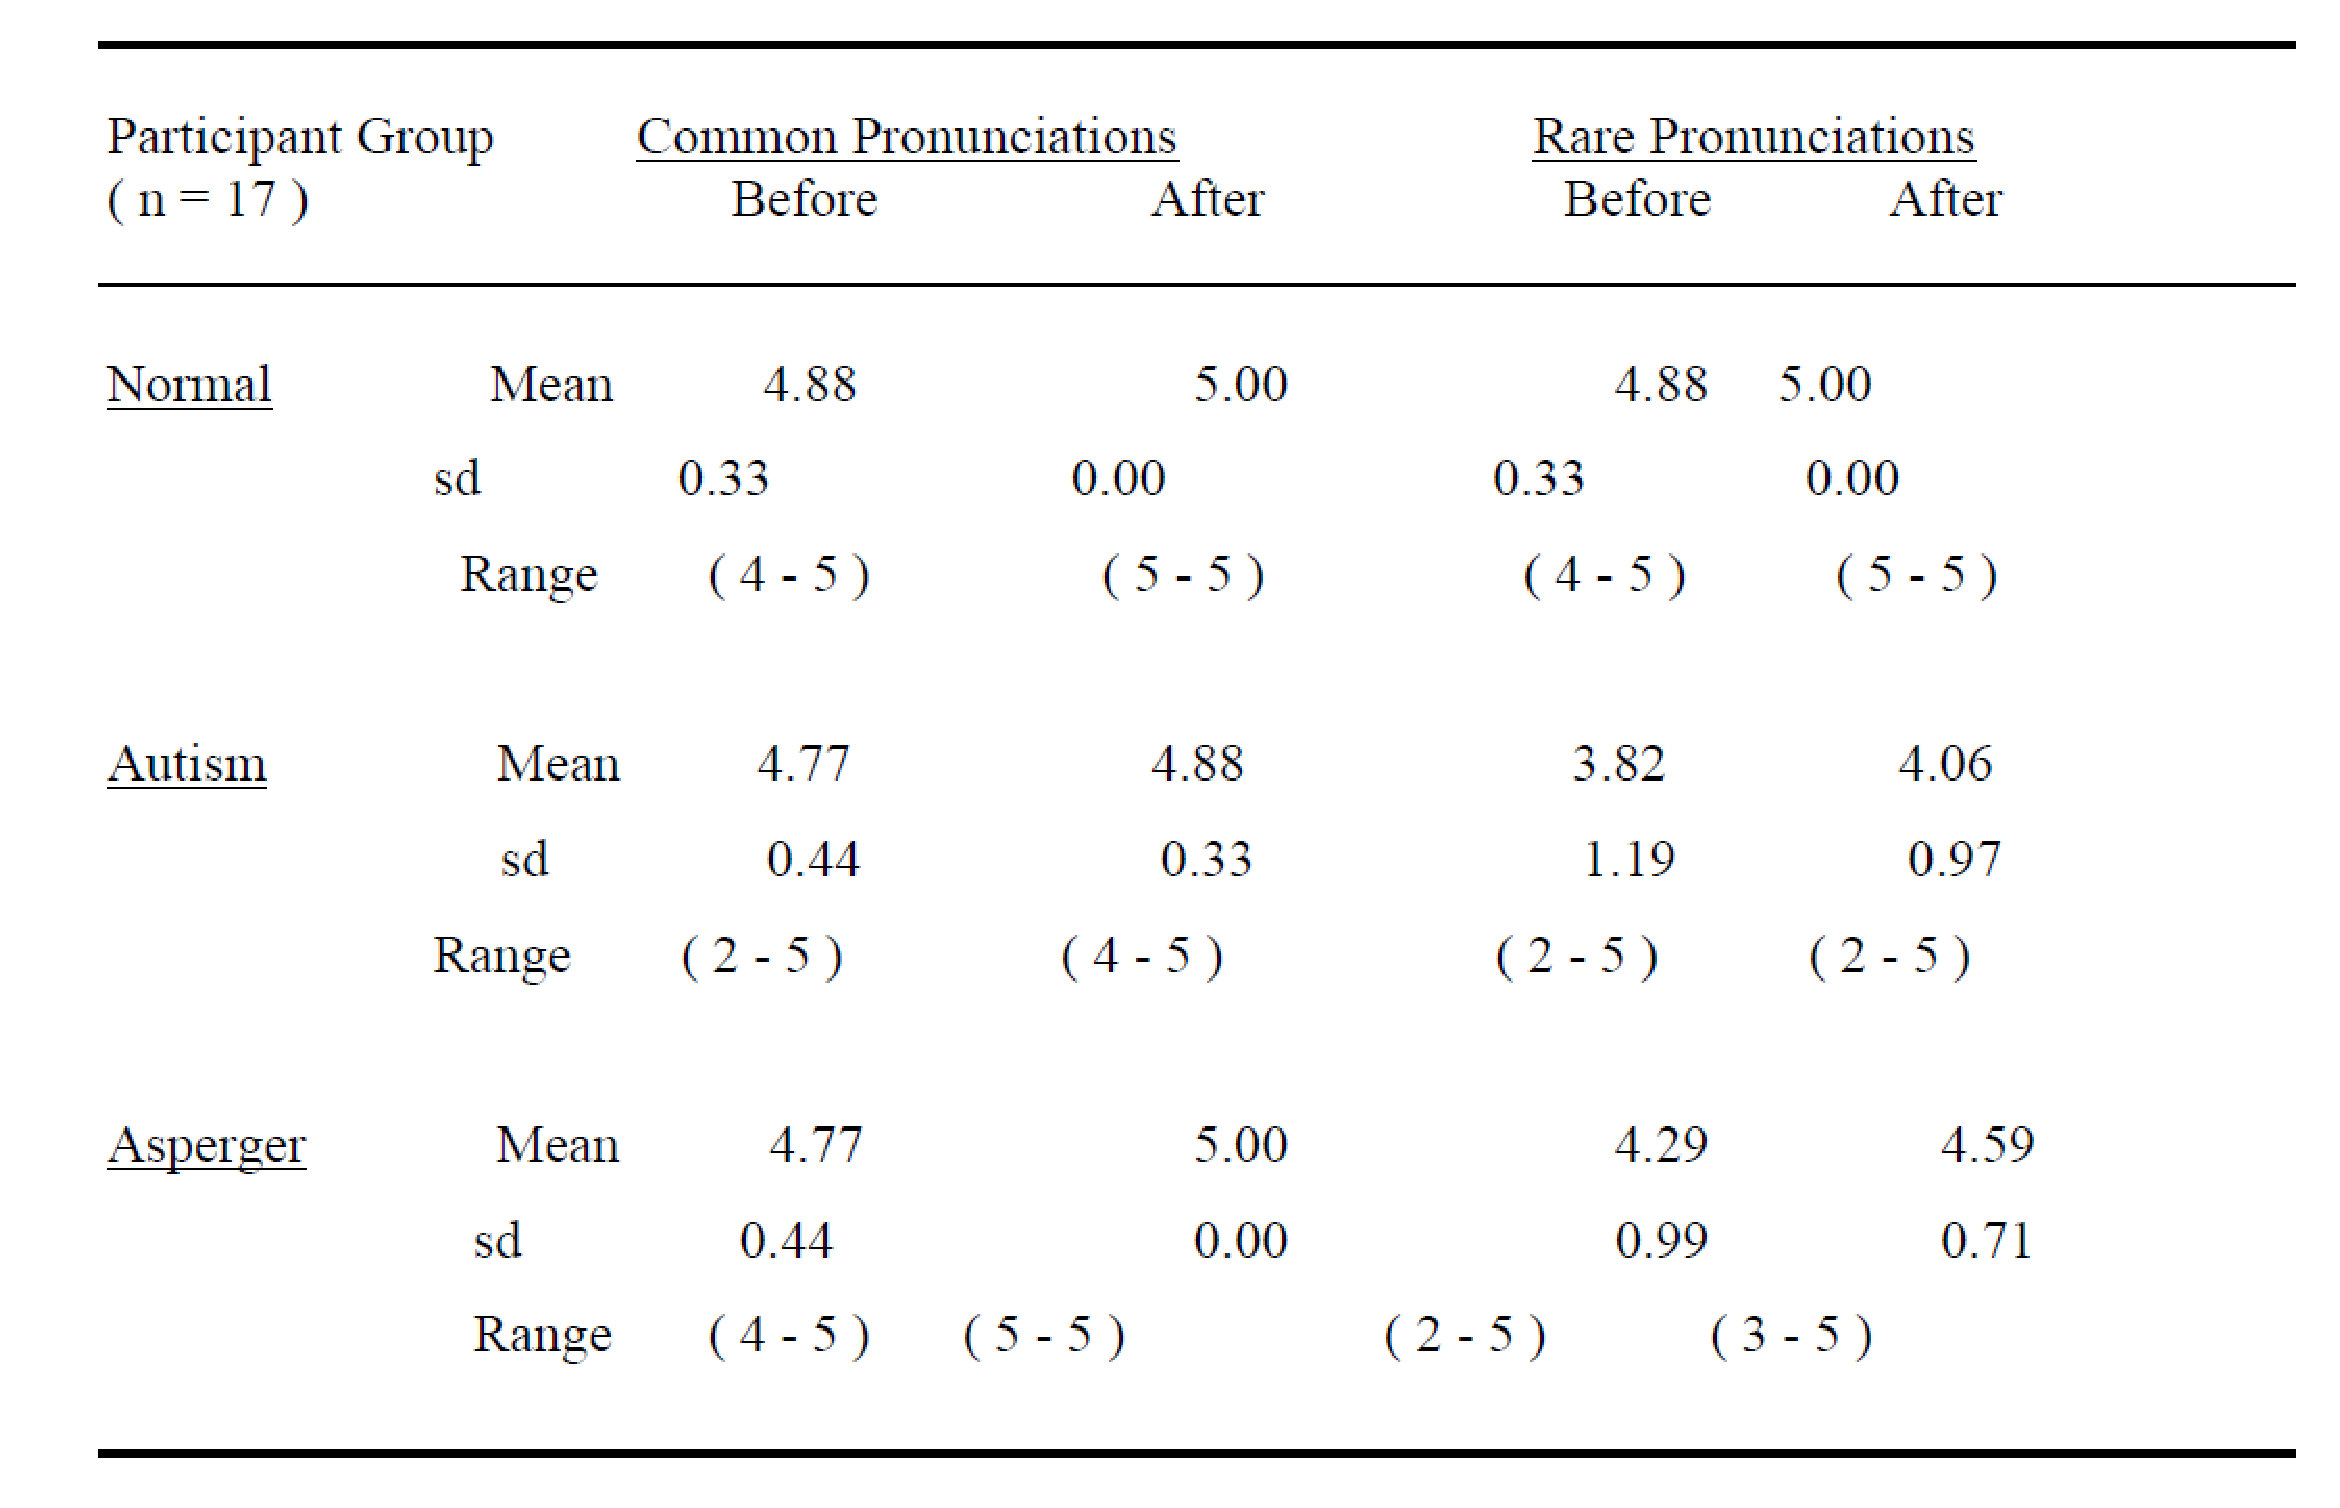
\includegraphics[width=115mm]{figures/asd_lexamb_study_results.eps}
\end{center}
\caption{Results from study on lexical disambiguation in people with ASD.  Common Before/After refers to a common interpretation of the homograph, and it occurring Before/After the contextual information respectively.  Similarly, Rare Before/After refers to a rare interpretation of the homograph, and it occurring Before/After the contextual information respectively.  Table from Jolliffe and Cohen (1999).}
\label{asd-lexamb-study}
\end{figure} 

\begin{figure}[tp]
\begin{center}
	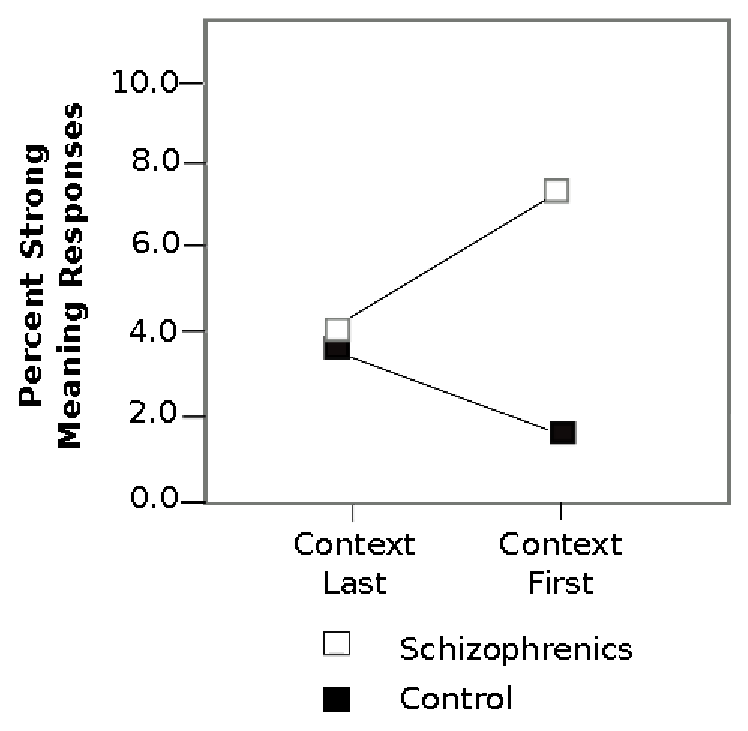
\includegraphics[width=100mm]{figures/schiz_lexamb_study_results.eps}
\end{center}
\caption{Results from study on lexical disambiguation in people with Schizophrenia.  Y-axis shows percentage of errors using the most common interpretation of the homograph, when the rare interpretation was correct.  Figure adapted from Cohen and Servan-Schreiber (1992).}
\label{schiz-lexamb-study}
\end{figure} 

\subsection{Modeling Lexical Disambiguation Effects in Autism}

\subsubsection{A Model of Word Sense Disambiguation}
The connectionist model utilized in Cohen and Servan-Schreiber (1992) was modified to investigate lexical disambiguity in people with autism and schizophrenia. (See Figure~\ref{cohen-servan-schreiber-model}.)  A localist code is used to represent words as inputs to the network.  The input layer also contains words that are used as the contextual cues to assist the network in the disambiguation task.  The output of the network (the ``Meaning Output Module'' in Figure~\ref{cohen-servan-schreiber-model}), also uses a localist code to represent the various possible meanings of the network.  Specifically, one unit is used to represent the interpretation of the word ``BANK'' as a ``financial Institution'', and one unit for the alternative meaning ``area next to a river'', etc.  The context layer (labeled ``Discourse Module'' in Figure~\ref{cohen-servan-schreiber-model}), was modified from its original version.  The original ``Discourse Module'' uses hand coded representations to encode sentential context information, meaning the very important process of learning representations which facilitate the integration of previous experience is hard wired.  we replaced the original ``Discourse Module'' version with a SRN layer, allowing the network to learn how to integrate temporally extended information through repeated experience. (See Figure~\ref{lexamb-model-task}.) 

\begin{figure}[tp]
\begin{center}
	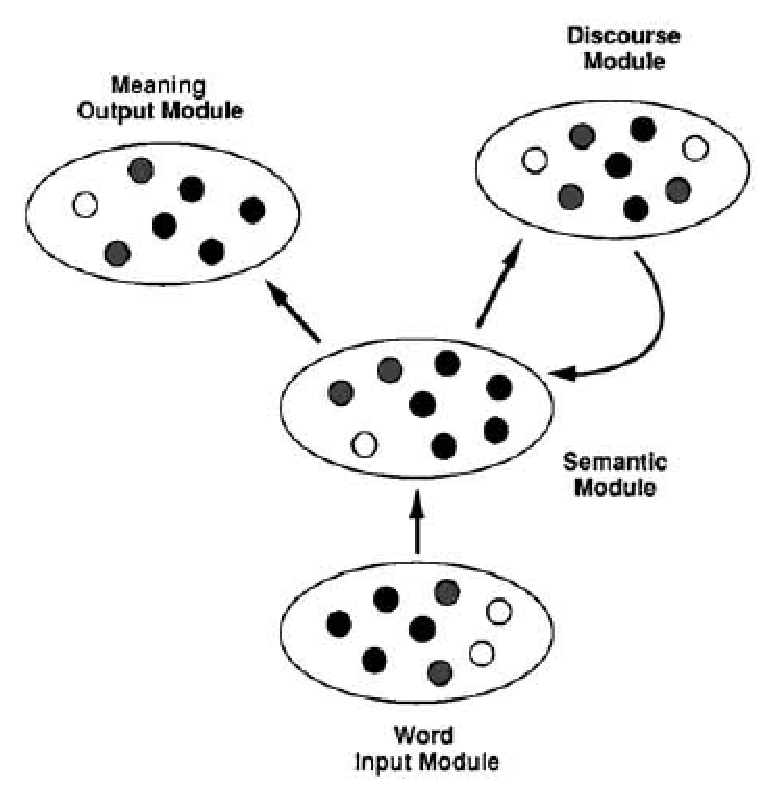
\includegraphics[width=100mm]{figures/Cohen_ServanSchreiber_Model.eps}
\end{center}
\caption{The original lexical ambiguity model. Image adapted from Cohen and Servan-Schreiber (1992).}
\label{cohen-servan-schreiber-model}
\end{figure} 

\subsubsection{Training}
The corpus used for training involved 50 input units representing 50 ambiguous homographs.  Also used as input to the network was 50 disambiguating context units.  Two context units were assigned to each of the 50 homograph units, resulting in each homograph unit being paired with two different context units. Also, each context unit is paired with two different homograph units, ensuring that every context unit is involved in two completely different disambiguation trials.  Setting up the input corpus in this manner prevents the network from learning a one-to-one association of a context unit to a specific homograph word meaning, removing any possibility that the network could solve the task while ignoring all of the homograph units, instead relying only on the information provided by the contextual units to disambiguate the meaning of a homograph.  One context unit was used for the more frequent use (strong) and one unit for the less frequent (weak) use of each homograph.  This will results in 150 possible outputs for the network (100 possible homograph interpretations and 50 context words used for disambiguation of the homographs).  Each possible output can be thought of as representing the proper ``meaning'' input words presented to the network.  (See Figure~\ref{lexamb-model-task}.)  %The network also used 100 units each within the Hidden layer and the Context Layer, it should be noted, however, that varying this value had little effect on the networks overall performance.

One word (input unit) is presented to the network at a time, requiring the network to make a response to every word independent of whether the input is supplied via a contextual or homograph unit.  On each trial, the network is presented with a mini-clause consisting of three words, including a context/homograph pair followed by a homograph probe. The pieces of each mini-clause should be thought of as representing the sentences presented to the subjects in the original study (the context and homograph units), followed by questioning the subjects on the meaning of the ambiguous word (the probe homograph unit).  The order of presentation for the context and homograph units were counterbalanced across all trials, ensuring equal experience with utilizing context at both the beginning and the end of mini-clauses.  The final probe homograph unit was always presented last, and was needed to assess if the network could properly disambiguate the meaning of the homograph after reading the mini-clause.  The network was trained to respond with the correct ``meaning'' for both input types, homograph and context units, by activating a single unit within the output layer which represents the proper semantic interpretation of the input word presented to the network. (See Figure~\ref{lexamb-model-task}.) The network was presented with the strong interpretation of the homographs on 70\% of the trials and the weak interpretation on 30\%.

\subsubsection{Testing}
The same testing procedures as Cohen and Servan-Schreiber (1992) were utilized.  The model was presented with a context and ambiguous word unit pair, one unit at a time.  The order of presentation was again counterbalanced across all testing trials.  After the presentation of the pair, the model was presented with the probe ambiguous homograph word unit.  Note that these are the same ``mini-clauses'' that were utilized throughout the training procedure. The main measure of interest is percentage of incorrect uses of the strong interpretation by the model during the presentation of the probe homograph unit, when the weak interpretation is correct based on the context provided in the mini-clause.  The results were separated into two groups, ``Context Presented First'' and ``Context Presented Last'' to enable comparison to the human subjects data.

\begin{figure}[tp]
\begin{center}
	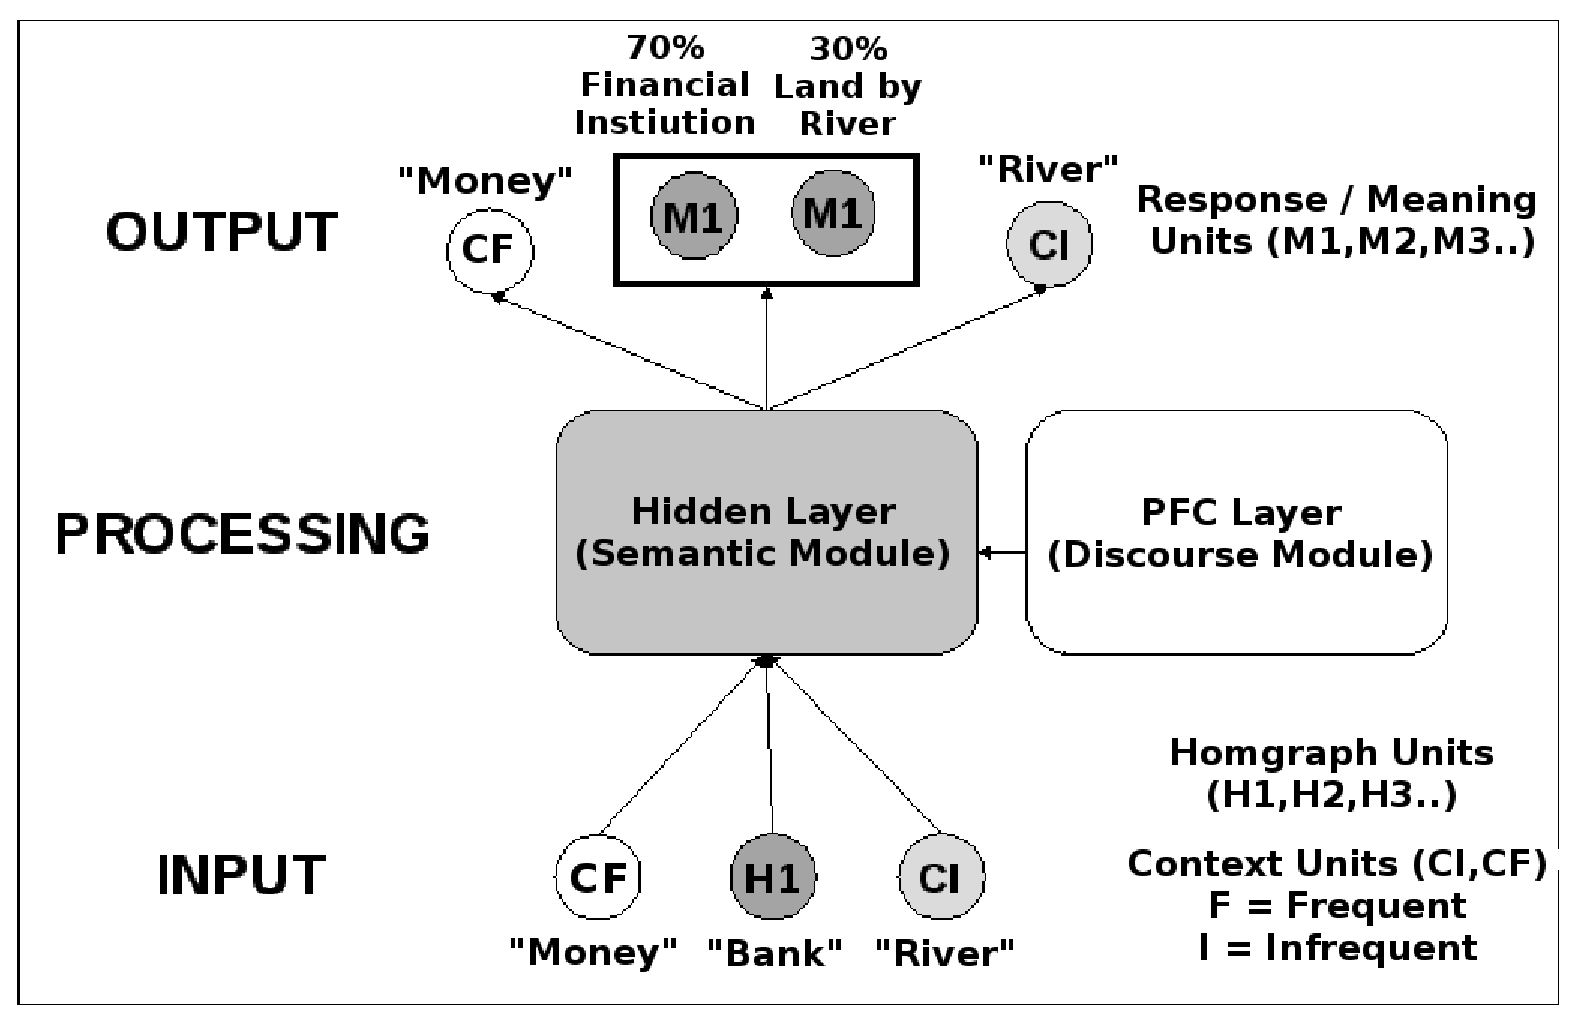
\includegraphics[width=115mm]{figures/lexAmb_network_cartoon.eps}
\end{center}
\caption{Cartoon of the lexical ambiguity model and task.  The task of the model is to correctly respond to any input word presented within the ``INPUT'' layer of the network by activating the unit representing the appropriate meaning at the ``OUTPUT'' layer of the network.  The context units are used to disambiguate the meaning of a specific homograph unit.  Words are presented to the network one at a time and it is the networks job to learn, through experience, to respond with the correct meaning via the ``OUTPUT'' layer of the network.}
%For instance, in this figure the ambiguous homograph input unit represents the word ``Bank'' and the frequent and infrequent context input units represent ``Money'' and ``River'' respectively.  When the infrequent context unit ``River'' is presented first to the network followed by the homograph unit for ``Bank'', the network was expected to learn to use the context unit's meaning to correctly respond ``Land by River''.  This response occurs during the final trial when the network is probed for the correct meaning of the ambiguous homograph unit after the initial mini-clause has been presented.}

\label{lexamb-model-task}
\end{figure} 

\subsubsection{Modeling Schizophrenia}
%We employed the same mechanism used by Cohen and Servan-Schreiber to model the effects of different levels of tonic dopamine on neural processing.  Namely, lowering the gain parameter on modeled neurons within the context layer of the model after initial training has taken place.   Figure~\ref{gain-manipulation} shows the overall effect of this manipulation.  As the gain parameter is increased, the overall effect of the input is heightened.  As the gain decreases, on the other hand, the effect of the net input decreases.  This is believed to mimic the potentiating effects of dopamine on target neurons.  
In the original model of schizophrenic performance of Cohen \& Servan-Schreiber, a hypothesized tonic DA deficit was instantiated by reducing the gain of the activation function on all modeled PFC units. Figure~\ref{gain-manipulation} shows the overall effect of this manipulation.  Coupled with the dynamics of the network, the result was a less stable PFC representation of the contextual information.  Thus, if the context were to come at a point temporally distant from homograph ``probe'', the contextual information maintained within the modeled PFC was more likely to degrade and be of little use to the network.  However, if the context was presented temporally close to the``probe'', the contextual information maintained within the PFC could still be used to disambiguate the meaning.  This manipulation successfully matched the pattern of behavior seen in schizophrenia.  Functionally analogous to the gain manipulation of Cohen \& Servan-Schreiber, we systematically reduced the ability of the Context Layer (PFC) to hold on to information over an extended period of time in order to model the performance of people with schizophrenia.  By systematically reducing the parameter that controls the amount of previous Context Layer activity retained from time step to time step, we can functionally reduce the stability of the contextual representations maintained within the modeled PFC.  This manipulation provides an extremely close approximation to the gain reduction performed by Cohen \& Servan-Schreiber.   Also, schizophrenia most often emerges after a significant amount of development has occurred, therefore this deficit was only instantiated after the network had been trained to criterion.  In the healthy model, the context maintenance parameter is set to ensure that 30\% percent of the previous Context Layer's activation was retained from the previous time step.  In order to investigate schizophrenic behavior we reduced this parameter to 20\%, 10\%, and 0\%, systematically destabilizing the modeled PFC Layer's maintained pattern of activity. 
%Under normal circumstances, the Context Layer has the ability to effectively hold onto previous information over multiple time steps.  In a standard SRN, a complete copy of the previous time steps Hidden Layer activity pattern is copied directly into the Context Layer upon every time step.  However, within the Leabra framework there are two mixing parameters responsible for allocating what percentage of the activation is a pure copy of the previous Hidden Layer activity and what percentage is maintained from the previous state of the Context Layer itself.  These parameters can be seen as manipulating how well the network updates the contents of the PFC and how well the network can actively maintain this information within the PFC respectively.  By systematically reducing the parameter that controls the amount of previous Context Layer activity retained from time step to time step, we can functionally reduce the stability of the contextual representations maintained within the modeled PFC.  This manipulation provides an extremely close approximation to the gain reduction performed by Cohen \& Servan-Schreiber.   Also, schizophrenia most often emerges after a significant amount of development has occurred, therefore this deficit was only instantiated after the network had been trained to criterion.  In the healthy model, the context maintenance parameter is set to ensure that 30\% percent of the previous Context Layer's activation was retained from the previous time step.  In order to investigate schizophrenic behavior we reduced this parameter to 20\%, 10\%, and 0\%, systematically destabilizing the modeled PFC Layer's maintained pattern of activity. 

\begin{figure}[tp]
\begin{center}
	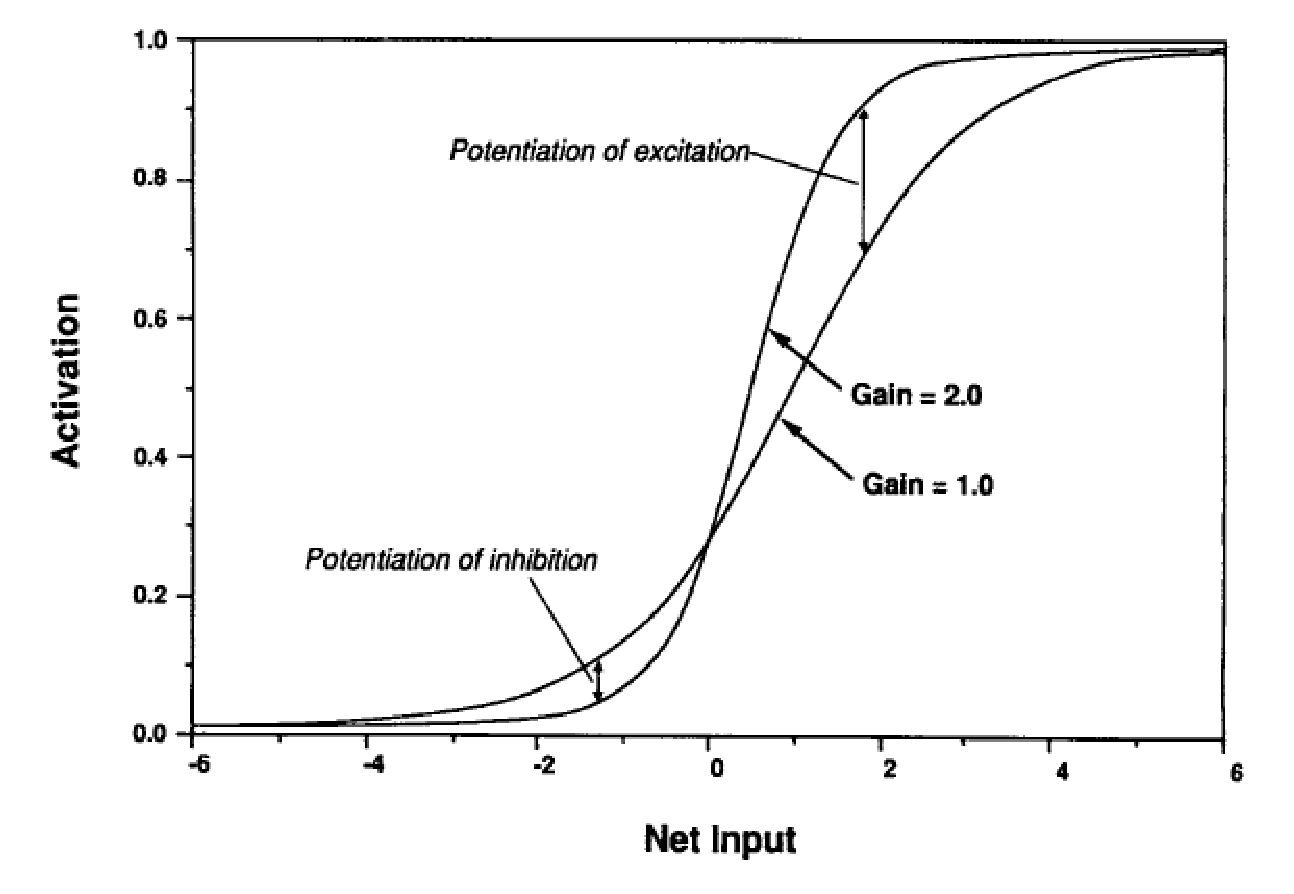
\includegraphics[width=100mm]{figures/gain_manipulation.eps}
\end{center}
\caption{Modeled effects of tonic DA on a standard activation function. An increase in the amount of DA heightens the effects of the net input, effectively increasing the signal-to-noise ratio in the network, while lower DA decreases the effects, reducing the signal-to-noise ratio. Image adapted from Cohen and Servan-Schreiber (1992).}
\label{gain-manipulation}
\end{figure} 

\subsubsection{Modeling Autism}
%In order to model the performance of people with autism, we propose to hinder the updating of the SRN context layer of the network as discussed previously.  Specifically, two distinct manipulations will be tested.  The first method will consist of gaussian noise being injected directly into the context layer of the SRN, resulting in contextual information which has been corrupted to varying degrees, based upon the amount of noise utilized.  In the second manipulation we will titrate the probability that the context layer is updated, mimicking a deficit flexible updating of the contents contained within the PFC.  This manipulation of the model is consistent with my proposed theory of impaired input and output gating of representations maintained within the PFC driven by DA interactions.  Importantly, this deficit will be instantiated from the beginning of development.  This is different than the modeled deficit proposed in Schizophrenia by Cohen and Servan-Schreiber, where the DA manipulation occurs after the task has been learned.   By instantiating a deficit in the context layer, the model may not be able to rely on temporally distant information, and, instead, must use the statistical regularities that are available at each time step.  The result should create a response bias towards the more frequently experienced words and a general inability to utilize context, as is observed in people with autism.

In order to model the performance of people with autism, we restricted the probability of successfully updating the Context Layer (PFC) upon each input presentation.  Specifically, we investigated successful PFC update probabilities of 100\% (control), 90\% and 80\%.  Preventing the updating of the PFC in this manner causes the temporally extended information normally contained within this layer to be much less reliable, making the learning of the sentential context difficult for the model to accomplish.  Without a reliable contextual representation of the previously presented information, the model will be forced to rely heavily the statistical frequency of the input corpus in order to learn the task.  Importantly, autism is believed to be a developmental disorder, with key neural differences likely present from very early on or even since birth.  To capture this fact, we restricted the ability of the modeled PFC layer to update throughout the entirety of training, simulating the deficit existing throughout key developmental periods.

\subsection{Lexical Dysambiguation Simulation Results}

\subsubsection{Overview}
Network simulations were repeated 10 times in each of the experimental conditions, with initial synaptic weights randomized for each repetition.  Each network experienced the entire training corpus 20 times.  The training corpus contains every potential context word / ambiguous homograph word pair, for a total of 200 different ``mini-clauses'', 100 with the contextual word presented first and 100 with the homograph occurring first in the clause.  Each of the ``mini-clauses'' are presented in a random order during each of the 20 blocks of training.  Lateral inhibition within the Output layer of network strongly encouraged the network to respond with a single ``word''.  The unit with the highest overall activation level was used as the model's response.  The key error measure across all conditions is the number of errors committed when assigning meaning to the ambiguous probe word and is visually presented in Figures~\ref{Schiz-Amb-Results} and \ref{ASD-Amb-Results}. The higher this measure, the worse the models performed on the disambiguation task.  

\subsubsection{Schizophrenia Model Results}
The model of homonym reading in schizophrenia was able to qualitatively match the behavioral data and reproduce the seminal modeling results of Cohen \& Servan-Schreiber (1992). (See Figure~\ref{Schiz-Amb-Results}.)  The ``Control'' network performed well regardless of the frequency of the meaning word (``Rare'' vs.``Common'').   Also, the ordering of contextual information had virtually no effect on model performance.  The model performed well regardless of if the context was presented early in the mini-clause (Context-First) or if it came later (Ambiguous-First).  However, as the PFC representations were systematically destabilized the error rate rose significantly. Importantly, this decrease in task performance only occurred when the context was presented first, but not when the context was presented last.  (See Figure~\ref{Schiz-Amb-Results}.)  
%Two-way ANOVAs were performed separately on each destabilization level -- 0\% Destabilized (Control), 33\% Destabilized, 66\% Destabilized, and 100\% Destabilized --, with frequency (``Rare'' vs. ``Common'') and ordering (``Context First'' vs. ``Meaning First'') as factors.  An effect of frequency was observed as the PFC was destabilized 33\%, 66\%, and 100\% (respectively, F(1,36) = 18.29, p $< .05$; F(1,36) = 57.48, p $< .05$; F(1,36) = 78.98, p $< .05$).  Also, an effect of ordering was observed for each condition (respectively, F(1,36) = 14.97, p $< .05$; F(1,36) = 77.72, p $< .05$; F(1,36) = 109.42, p $< .05$). Importantly, a there was a significant frequency by ordering interaction effect in all cases where the PFC was destabilized (respectively, F(1,36) = 11.99, p $< .05$; F(1,36) = 54.84, p $< .05$; F(1,36) = 73.49 p $< .05$).  This supports the observation that only the context first error rate rose significantly as a result of PFC destabilization. No effects were found in the control network results for either frequency F(1,36) = .64, p $>.05$; or ordering F(1,36) = 3.47, p $>.05$, and the frequency by ordering interaction was also non-significant F(1,36) = 1.77, p $>.05$.  This matches patterns of behavior reported in previous schizophrenia research~\cite{CohenJD:1992:Schizophrenia}, which demonstrated that people with schizophrenia have difficulty utilizing context when it is presented temporally distal from the homograph it is intended to disambiguate.    
%Two-way ANOVAs were performed separately on each destabilization level -- 0\% Destabilized (Control), 33\% Destabilized, 66\% Destabilized, and 100\% Destabilized --, with frequency (``Rare'' vs. ``Common'') and ordering (``Context First'' vs. ``Meaning First'') as factors.  An effect of frequency was observed as the PFC was destabilized 33\%, 66\%, and 100\% (respectively, F(1,36) = 18.29, p $< .05$; F(1,36) = 57.48, p $< .05$; F(1,36) = 78.98, p $< .05$).  Also, an effect of ordering was observed for each condition (respectively, F(1,36) = 14.97, p $< .05$; F(1,36) = 77.72, p $< .05$; F(1,36) = 109.42, p $< .05$). Importantly, a there was a significant frequency by ordering interaction effect in all cases where the PFC was destabilized (respectively, F(1,36) = 11.99, p $< .05$; F(1,36) = 54.84, p $< .05$; F(1,36) = 73.49 p $< .05$).  This supports my observation that only the context first error rate rose significantly as a result of PFC destabilization. No effects were found in the control network results for either frequency F(1,36) = .64, p $>.05$; or ordering F(1,36) = 3.47, p $>.05$, and the frequency by ordering interaction was also non-significant F(1,36) = 1.77, p $>.05$.  This matches patterns of behavior reported in previous schizophrenia research~\cite{CohenJD:1992:Schizophrenia}, which demonstrated that people with schizophrenia have difficulty utilizing context when it is presented temporally distal from the homograph it is intended to disambiguate.    

\subsubsection{Autism Model Results}
By restricting the ability of the Context Layer to update in a flexible manner, we was able to capture patterns of behavior consistent with previous findings of lexical disambiguation research in people with ASD~\cite{RefWorks:103,HappeF:1997:WCC_Homographs}. (See Figure~\ref{ASD-Amb-Results}.) Specifically, as the probability of updating the content of the modeled PFC layer was systematically reduced, the network became increasingly more reliant on the statistical frequency of the words.  Behaviorally this was manifested in a significantly higher error rate when the model needed to utilize contextual information, \emph{regardless of the temporal distance from the required response}, in order to correctly interpret the ``Rare'' meaning of the homograph in the sentence.  These results suggest that the model of autistic performance has difficulty utilizing contextual information to overcome a more frequent interpretation of a homograph, regardless of when it is presented in the sentence.  (See Figure~\ref{asd-lexamb-study}.) 
%Two-way ANOVAs were performed separately on each level of PFC updating  -- 100\% probability to update PFC (Control), 90\% probability to update PFC, and 80\% probability to update PFC -- with frequency (``Rare'' vs. ``Common'') and ordering (``Context First'' vs. ``Meaning First'') as factors.  An effect of frequency was observed in the ``autistic-like'' condition, where the PFC is restricted to update only 90\% and 80\% of the time (respectively, F(1,36) = 64.52, p $< .05$; F(1,36)=116.58, p $< .05$). However, an effect of ordering was not observed (respectively, F(1,36) = 0.35, p $> .05$; F(1,36) = 0.31, p $> .05$). Also, the frequency by ordering interaction was not significant in either case (respectively, F(1,36) = 0.87, p $. .05$; F(1,36) = 0.31, p $> .05$). These results suggest that the model of autistic performance has difficulty utilizing contextual information to overcome a more frequent interpretation of a homograph, regardless of when it is presented in the sentence.  No effects were found in the control network results for either frequency F(1,36) = .64, p $>.05$; or ordering F(1,36) = 3.47, p $>.05$, and the frequency by ordering interaction was also non-significant F(1,36) = 1.77, p $>.05$.  It is important to note that as the probability of updating the Context Layer was reduced, the model of autistic behavior performed worse overall when compared to the control network, including common interpretations of the homographs.   This pattern was not reported in the behavioral study of people with ASD.  However, the extremely low number of sentences in each condition (5) may be resulting in ceiling effects, limiting the ability to reliably detect this difference in their sample. (See Figure~\ref{asd-lexamb-study}.) 

%\& Servan-Schreiber (1992). See Figures~\ref{Schiz-Amb-First} \& \ref{Schiz-Context-First}.)  The ``Control'' network performed well regardless of the frequency of the meaning word (``Rare'' vs.``Common'') as well as if the contextual information came early in the mini-clause(Context-First) or if it came later (Ambiguous-First).  However, as the PFC representations were systematically destabilized (as is hypothesized to occur in schizophrenia due to tonic-DA dysfunction), the error rate rose significantly for when the context was presented first, but not when the context was presented last.  This matches patterns of behavior reported in previous schizophrenia research~\cite{CohenJD:1992:Schizophrenia}
%Also, the model added to the original modeling effort by allowing the contextual representations in the modeled PFC be learned from experience, instead of being hand-coded by the modeler.



\begin{figure}[tp]
\begin{center}
	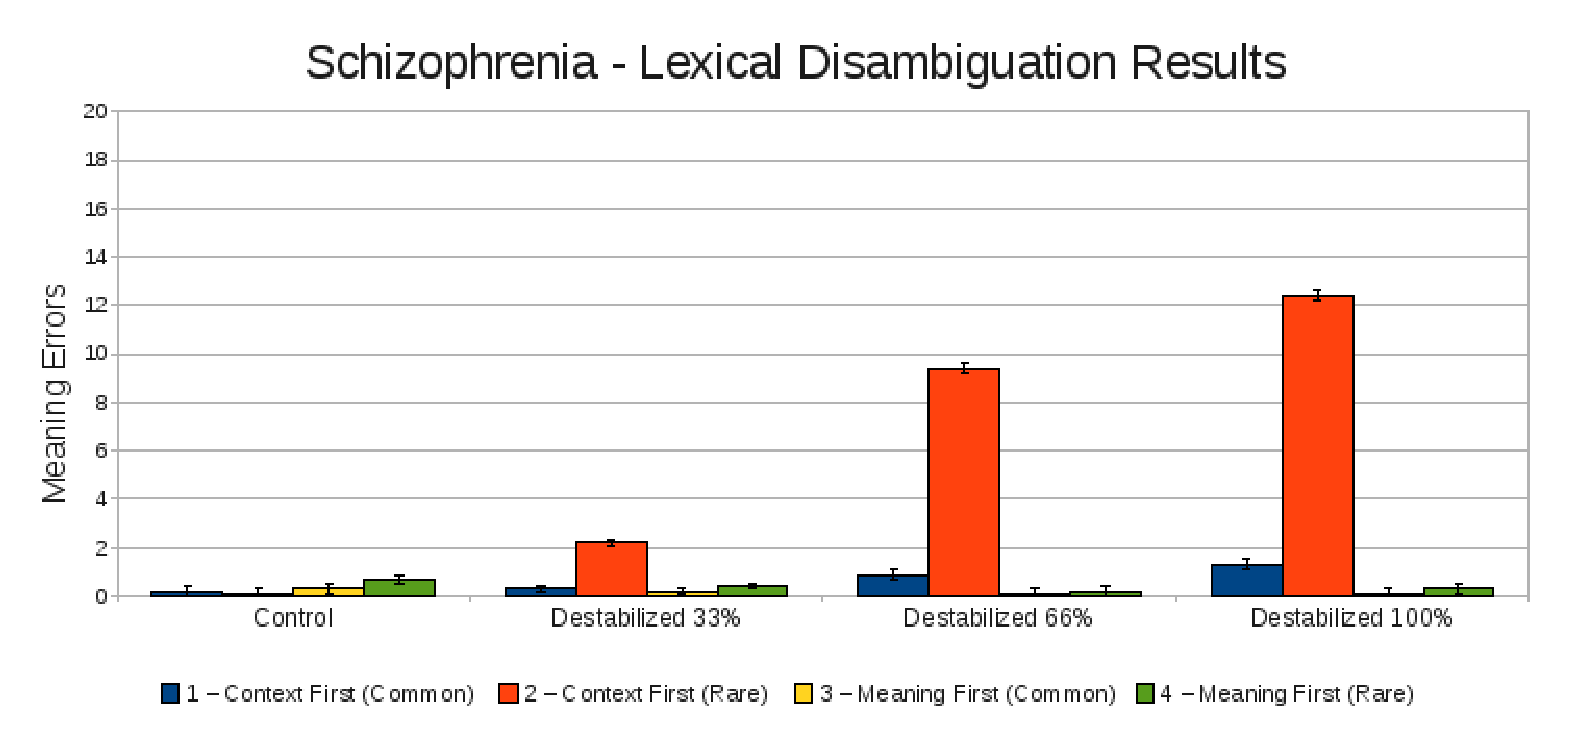
\includegraphics[width=140mm]{graphs/schiz_lexamb_results.eps}
\end{center}
\caption{Schizophrenia Model Results. As the modeled PFC is destabilized, the model performs selectively worse on condition (2).  In this condition the contextual information is presented first and the model must use this information to override the more common interpretation of the homograph. } 
\label{Schiz-Amb-Results}
\end{figure} 

\begin{figure}[tp]
\begin{center}
	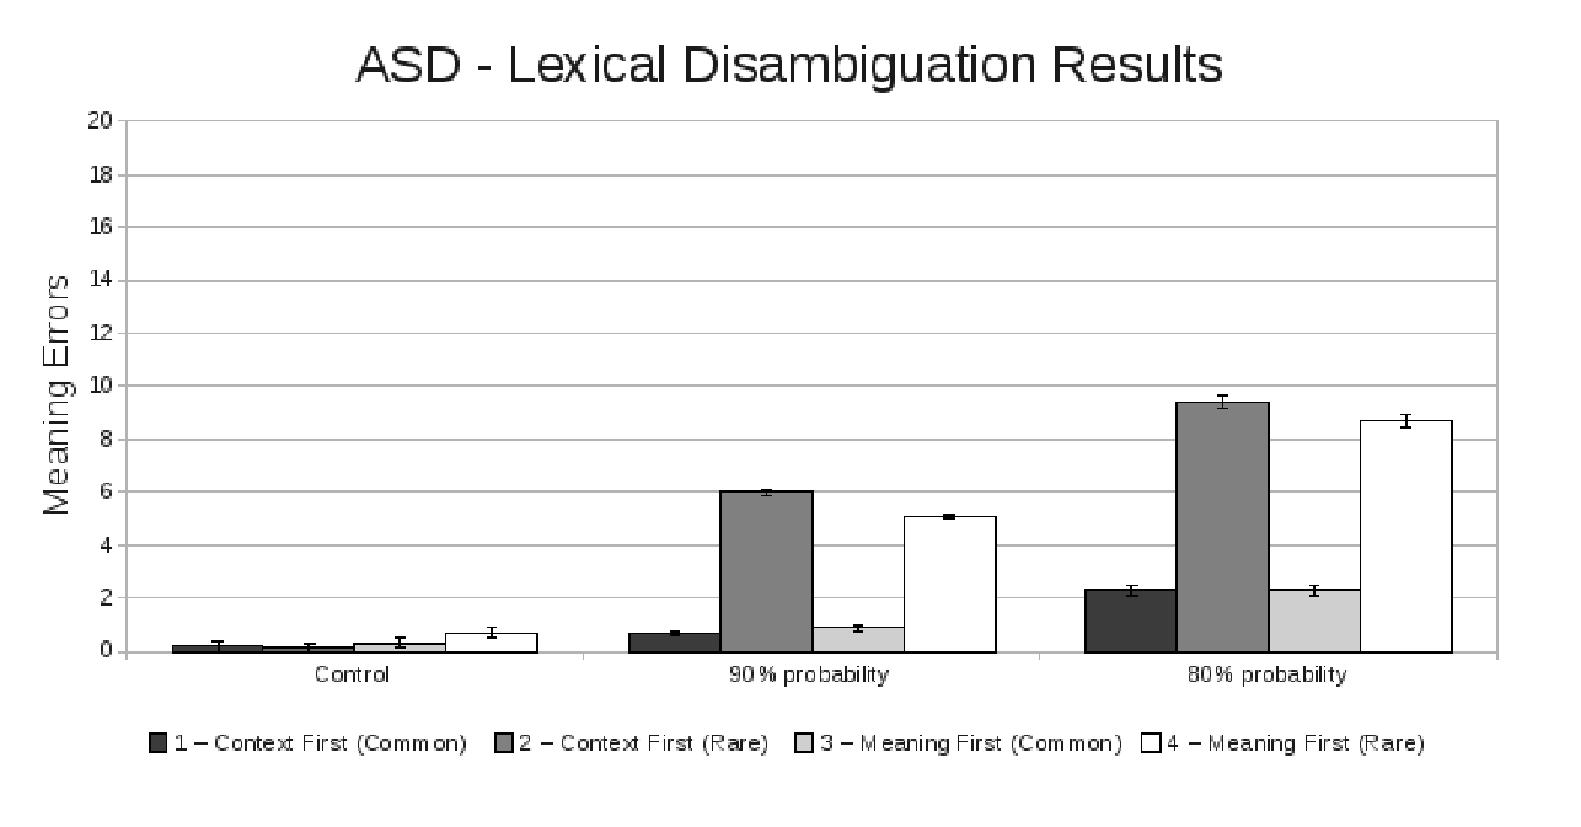
\includegraphics[width=140mm]{graphs/asd_lexamb_results.eps}
\end{center}
\caption{ASD Model Results. Systematically reducing the ability of the modeled PFC to update its contents resulted in worse performance on conditions (2) and (4).  These are the conditions that require the use of contextual information in order to override the more common interpretation of the homograph. } 
\label{ASD-Amb-Results}
\end{figure} 

%\subsection{Summary}
%In this chapter modeling results were presented demonstrating how a specific neural difference, dysfunctional interactions between the mid-bran DA system and PFC, can capture patterns of dysfunction in people with autism when utilizing sentential context to disambiguate the meaning of homographs.  Our work suggests that improper DA / PFC interactions lead to problems flexibly updating the contents of the PFC, and difficulties arise due to the lack of reliable contextual representations.  This causes the model to rely more heavily on statistical regularities in the environment.  In other words, the model adopts a policy of responding with the most common interpretation of a homograph in order to minimize errors, in lieu of appropriate contextual guidance from the Context Layer.  A previously published and theoretically justified computational model of lexical disambiguation was modified in a manner consistent with my hypothesis in order to capture the behavior of people with autism~\cite{CohenJD:1992:Schizophrenia}.  Interestingly, the Cohen \& Servan-Schreiber model was originally developed as an investigation into lexical disambiguation difficulties in people with Schizophrenia.  This provided my investigation with an interesting clinical comparison group, especially considering the qualitatively different behavioral profiles of the two disorders coupled with the suggestion of DA dysfunction underlying each respective pattern.  By positing the disorders actually have different \emph{kinds of DA dysfunction}, namely tonic DA dysfunction in schizophrenia and phasic DA abnormalities in ASD, the model is capable of explaining both the original findings of Cohen \& Servan-Schreiber and the patterns of behavior found in people with ASD~\cite{RefWorks:103,HappeF:1997:WCC_Homographs}.  

